\subsection{End-to-End Results}
\label{sec:exp-e2e-results}

%1. overview & metric (3 sents)
Now we perform the cross-lingual table linking experiment and compare with
previous table linking and text linking systems.
Recap that not all mentions in our dataset have a gold English entity.
we only attempt to link those mentions with English labels (see Definition \ref{def:mention}).
%For mentions not to be linked,  are still helpful for the mention is still helpful, since it
%and exclude mentions  without a proper Chinese concept,
%or failed to transfrom into the equaivalent English concept.
To be consistent with state-of-the-art systems, we report Micro Accuracy
and Macro Accuracy as the evaluation metrics.
Micro Accuracy, used in $TabEL_B$~\cite{bhagavatula2015tabel} and
$TabEL_W$~\cite{wu2016entity}, is the fraction of cells
where the predicted entity exactly matches the labeled English concept.
We also adopt Macro Accuracy, defined as the fraction of
correctly linked cells averaged over all tables, this metric
avoids the results biased the table with more cells.

%2. show result, overall statement (3 sents)

In order to keep a fair comparison,
due to both $TabEL_B$ and $TabEL_W$ taking only one English mention per cell as the input,
we select Baidu translation as the best one (see \secref{sec:exp-cand-gen-eval})
and apply this translation setting to all approaches.
In addition, we evaluate our approach under the full translating strategy,
using either pre-train or without pre-train.
For all the variations of our approach,
we fix $N_{cand}=30$, $N_{tab}=49$, $d_{cell}=d_{cont}=100$, $d_{out}=200$, $\eta=0.0002$ and $l_1=l_2=0.0005$, 
as reaching the highest Micro Accuracy in the validation set.
Whereas we use different $N_{cand}$ for the other approaches, tuning separately.

We report the experimental results in \tabref{tab:main-result}.
For the 4 experiments using Baidu translation only, 
Our model outperforms the other baseline models, improving the result by up to 13.7\%.
Our full model even improves the Micro Accuracy by an absolute gain of 0.048,
showing the importance of combining multiple translating tools.
Besides, the pre-train module also plays an important role in our approach,
raising the Micro Accuracy by 0.03.
%3. compared with TabEL, ()
Both $TabEL_B$ and $TabEL_W$ suffers from the problem of error propagation
in the translating step, as the mono-lingual approaches take translated mentions
as direct input, a poor translating quality harms the final result.
Whereas our approach takes Chinese mention as the input, such end-to-end approach
alleviates the error brought by translation.
%4. compared with Wu
%Compare our approach with $TabEL_{Ch}$, it's no suprise to observe that,
%the mono-lingual table linker keeps competitive under the perfect translation
%of Wiki concepts from Chinese to English, but the gap between theirs and our approach
%(xx.x versus xx.x) is relatively small.
%\KQ{So shall we add another experiment? Use Wiki-inter-link to generate candidates ?}
%5. compare with text EL (Wiki inter-link, ours)
%6. Summary


%We show the experimental results in \tabref{tab:main-result}.
%Our model outperforms previous work and improves the acurrency by a relative gain of xx\%.
%For TabEL, the linking accuracy is limited by the quality of translated English table.
%By manually inspecting the translated English mentions, the translation accuracy is around xx\%,
%which is close to our quality of English candidate generation in \secref{sec:cand-gen-eval}.


\begin{table}[ht]
\centering
\caption{Experimental results on Chinese table linking task.
All baseline approaches take Baidu as the only translating tool.}
\label{tab:main-result}
\begin{tabular} {c|c|cc}
    Approach          & Micro Acc.   & Macro Acc.    \\
    \hline
    $TabEL_B$         &  0.513       & 0.511         \\
    $TabEL_W$         &  0.517       & 0.521         \\     %N_{cand} = 10
    $TextEL$          &  0.476       & 0.465         \\
    Ours (Baidu Only) &  0.588       & 0.583         \\
    \hline
    Ours (Full, w/o pre-train) &  0.606    &  0.591        \\ 
    Ours (Full, w/ pre-train)  &  \textbf{0.636}       & \textbf{0.630}         \\
\end{tabular}
\end{table}

We further analyze how the candidate size of a mention effects the table linking result.
The intuition is that, when $N_{cand}$ goes larger, the upperbound of the final result increases,
however, with more negative candidates been introduced, it's more difficult for a linking
system to reach the upperbound.
Therefore, we perform the experiment under different candidate size and investigate how
does each model handle this tradeoff.

\figref{fig:main-result} shows the trend of each approach, using Baidu translation only.
We also display upperbound (Hits@$n$) in the figure.
From the results, we observe that the Micro Accuracy increases when $N_{cand}$ is small,
and then decreases when $N_{cand}$ goes larger.
Our approach and $TabEL_B$ keeps a stable performance with a subtle performance decreasing, 
while $TextEL$ drops dramatically, even if the candidate size is smaller than 10.
Two main reasons are:
1) the BLDA model is unsupervised, though equivalent articles between
Chinese and English Wikipedia pair together as the input documents, the model doesn't observe
any explicit (mention, entity) pair for learning,
2) the similarity between the mention and the entity is only determined by their topic
distributions, without features derived from entity names, or from coherence information.
These reasons make $TextEL$ much more sensitive to noisy candidates.
Compared with baseline systems, our approach is more adaptive to different size of candidates,
with less error propagation during the translation step,
and can produce promising end-to-end results.


\begin{figure}[th]
\centering
%\epsfig{file=fb-schema-4.eps, width=0.95\columnwidth}
\scalebox{0.25}{\includegraphics[angle=0]{main-result-crop.eps}}
\caption{Experimental results of Micro Accuracy varied from different size of candidates,
using Baidu translation only.}
\label{fig:main-result}
\end{figure}
